\documentclass{mi-seminar}

\usepackage{hyperref}
\usepackage{graphicx}
\usepackage[T1]{fontenc}
\usepackage[utf8]{inputenc}
\usepackage{ngerman}

\title{Flying Etiquette}
%\subtitle{Dokumentation zum Projekt Informationsvisualisierung}
\author{Kevin Angermeyer \\ \and Lydia Güntner \\ \and Maximiliane Windl}



\title{Flying Etiquette}
\author{Kevin Angermeyer, Lydia Güntner, Maximiliane Windl}
\semester{SS18}
\course{Projektseminar Mediengestaltung I: Informationsvisualisierung}
\module{MEI-M05.3 }
\dozent{Florin Schwappach}
\studid{1796468, 1785088, 1770307}
\studSemester{6. Semester B.A. Medieninformatik / Informationswissenschaft}


%\address{Domplatz 1, 93047 Regensburg}{} % Optional
\mail{kevin.angermeyer@stud.uni-regensburg.de, lydia-maria.guentner@stud.uni-regensburg.de, maximiliane.windl@stud.uni-regensburg.de}




\begin{document}

\maketitle
\vspace*{2.5cm}
\section{Das Projekt starten} \label{Das Projekt starten}
Um das Projekt zu starten muss \textit{Python} installiert sein.
\subsection{Unix}
\textbf{Wie wird das Projekt gestartet?}\newline
\begin{enumerate}
\item Über das Terminal zum Projekt navigieren
\item Im Projekt durch den Befehl \textit{python -m SimpleHTTPServer} den Server starten.\newline
\item Im Browser auf localhost:8000 wechseln.
\end{enumerate}
\subsection{Windows}
\textbf{Wie wird das Projekt gestartet?}\newline
\begin{enumerate}
\item Die Datei Run.bat mit Doppelklick in der Kommandozeile starten 
\item Im Browser auf localhost:8000 wechseln.
\end{enumerate}

\section{Datensatz} \label{Datensatz}
Bei dem Datensatz handelt es sich um den Datensatz \textit{flying-etiquette-survey} von \textit{\href{https://github.com/fivethirtyeight/data/tree/master/flying-etiquette-survey}{fivethirtyeight}}. Die Daten stammen aus einer Online-Umfrage, welche mit \href{https://www.surveymonkey.com/mp/audience/}{SurveyMonkey}, am 29. und 30. August 2014 durchgeführt wurde. Insgesamt nahmen 1040 Probanden an der Studie teil. Nach einer Säuberung der Daten, bei der alle Teilnehmer die angaben nie zu fliegen und daher die anderen Fragen zum Thema Fliegen nicht beantwortet hatten, entfernt wurden, blieben Daten von 856 Probanden übrig. 
\newline \newline
Anschließend wurde der Datensatz in verschiedene Kategorien aufgeteilt, denen folgende Fragen zugeordnet wurden:
\begin{enumerate}

\item demographischen Fragen:
\begin{itemize}
\item Gender
\item Age
\item Household income
\item Education 
\item Location
\item How tall are you? 
\item How often do you travel by plane? 
\newline \newline
\end{itemize}


\item auf Kinder bezogene Fragen:
\begin{itemize}
\item Do you have any children under 18?
\item In general, is it rude to bring a baby on a plane?
\item In general, is it rude to knowingly bring unruly children on a plane? 
\newline \newline
\end{itemize}


\item auf das Zurücklehnen der Sitze bezogene Fragen: 
\begin{itemize}
\item Do you ever recline your seat when you fly?
\item Is it rude to recline your seat on a plane? 
\item Under normal circumstances, does a person who reclines their seat during a flight have any obligation to the person sitting behind them? 
\item Given the opportunity, would you eliminate the possibility of reclining seats on planes entirely?
\newline \newline
\end{itemize}


\item auf den Sitzplatz bezogene Fragen: 
\begin{itemize}
\item In a row of three seats, who should get to use the two arm rests? 
\item In a row of two seats, who should get to use the middle arm rest?
\item Who should have control over the window shade?
\newline \newline
\end{itemize}


\item auf das Tauschen von Sitzplätzen bezogene Fragen: 
\begin{itemize}
\item Is it rude to ask someone to switch seats with you in order to be closer to friends?
\item Is it rude to ask someone to switch seats with you in order to be closer to family?
\item Is it rude to move to an unsold seat on a plane? 
\newline \newline
\end{itemize}


\item auf die Kommunikation mit anderen Fluggästen bezogene Fragen:
\begin{itemize}
\item Generally speaking, is it rude to say more than a few words to the stranger sitting next to you on a plane?
\item On a 6 hour flight from NYC to LA, how many times is it acceptable to get up if you're not in an aisle seat?
\item Is it rude to wake a passinger up if you are trying to go to the bathroom?
\item Is it rude to wake a passenger up if you are trying to walk around?
\newline \newline
\end{itemize}


\item auf im Flugzeug verbotene Dinge bezogene Fragen:
\begin{itemize}
\item Have you ever used personal electronics during take off or landing in violation of a flight attendant's direction?
\item Have you ever smoked a cigarette in an airplane bathroom when it was against the rules? 
\end{itemize}


\end{enumerate}

\section{Projektmanagement}
Zur Organisation des Projekts wurde die Plattform Github in Kombination mit Git verwendet. In einer der ersten Gruppentreffen, wurde der \textit{Issuetracker} mit \textit{Tickets} befüllt und geschätzt wie viel Zeit die einzelnen Tickets benötigen. 
Daraufhin wurde noch ein \textit{Project} auf Github angelegt mit den Spalten:
\begin{itemize}
\item \textbf{Queue: } Hier befinden sich alle \textit{Tickets}, die noch bearbeitet werden müssen
\item \textbf{Blocker: } Hier befinden sich alle \textit{Tickets}, die höchste Priorität haben, da diese den weiteren Fortschritt blockieren
\item \textbf{In Progress: } Hier befinden sich alle \textit{Tickets}, die gerade bearbeitet werden.
\item \textbf{Code Review: } Hier befinden sich alle \textit{Tickets}, für die ein offener \textit{Pull-Request} existiert, der von den anderen Projektbeteiligten angesehen werden muss.
\item \textbf{Needs Testing: } Hier befinden sich alle \textit{Tickets}, die getestet werden müssen.
\item \textbf{Queue: } Hier befinden sich alle \textit{Tickets}, die fertig sind.
\newline \newline
\end{itemize}
Offene \textit{Pull-Requests} wurden immer erst gemerged, wenn diese von einem anderen Projektmitglied angeschaut und akzeptiert wurden. 
In den wöchentlichen Gruppentreffen, wurden die \textit{Tickets}
auf die Mitglieder aufgeteilt.

\section{Startdiagramm}
Das Startdiagramm soll dem Nutzer ermöglichen, selbstständig sowie umfassend den Datensatz zu erkunden. Es besteht aus mehreren einzelnen Diagrammen, die zusammen als eine svg-Datei auf der Startseite dargestellt werden. Dadurch kann man auf einen Blick mehrere Aspekte des Datensatzes visuell abbilden. Ferner kann der Nutzer somit ohne Umwege mit einem Großteil der Daten interagieren. Der Unterschied zu den Bubble-Diagrammen auf den Unterseiten besteht darin, dass im Startdiagramm alle Aspekte des Datensatzes dargestellt werden, der Detailgrad und die Filteroptionen sind allerdings nicht in dem gleichen Ausmaß gegeben. Insgesamt besteht das Startdiagramm aus vier Segmenten (Äußerer Ring, Innerer Ring, Teilnehmer-Kreise und Info-Box), die zur besseren Übersicht in diesem Text einzeln erläutert werden. Eine statische Beschreibung über die Funktionen des Startdiagramms wurde über dem Diagramm zusätzlich eingefügt, um dem Nutzer zu erklären, welche Interaktionsmöglichkeiten er hat. Diese werden ebenfalls im Detail erläutert (Abbildung \ref{ScStartDiagram}).
\begin{figure}
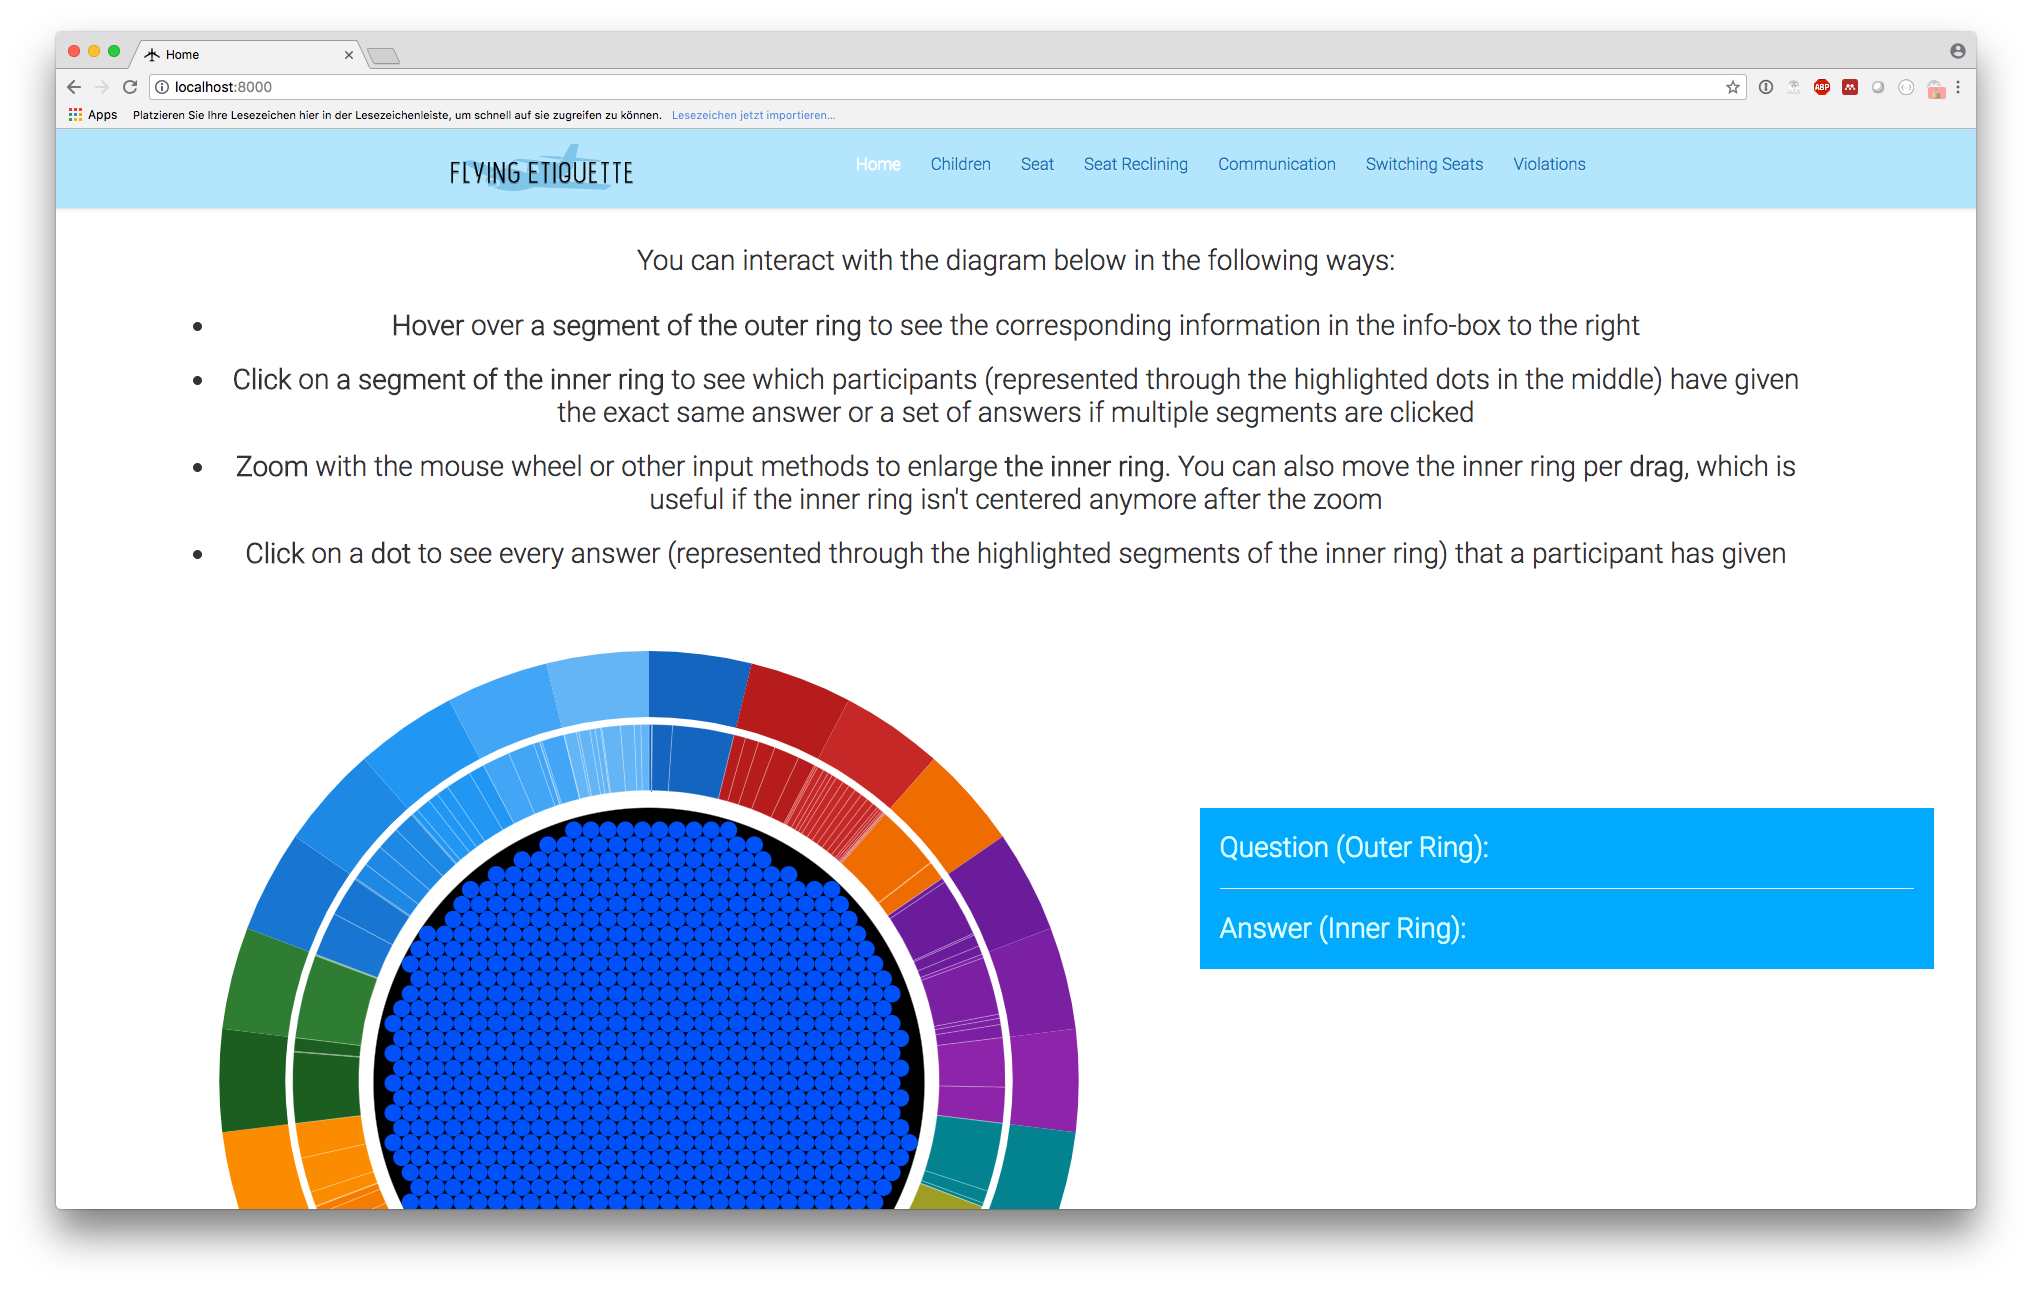
\includegraphics[scale=0.3]{assets/start_startpage.png}
\caption{Screenshot der Startseite \textit{Home} mit dem Startdiagramm inklusive dessen Beschreibung}
\label{ScStartDiagram}
\end{figure}

\subsection{Äußerer Ring}
Der äußere Ring wird durch ein Donut-Diagramm visualisiert und repräsentiert alle Fragen, welche die Teilnehmer der Studie beantworten sollten. Insgesamt 26 Fragen, die in \ref{Datensatz} nach den einzelnen Kategorien aufgelistet sind, wurden den Probanden gestellt. Jede Frage wird hierbei als ein Segment des äußeren Rings dargestellt. Jedes dieser Segmente erhält dabei zusätzlich noch eine Farbe, die abhängig von der Kategorie ist, in welche die Frage eingeordnet wurde. So sind z.B. alle auf Kinder bezogenen Segmente orange, während die demographischen Fragen hellblau sind. Fragen der gleichen Kategorie haben einen leicht anderen Farbton, um diese voneinander zu unterscheiden. 

Der äußere Ring hilft dem Nutzer auf einen Blick alle Fragen, sowie deren dazugehörige Kategorie mithilfe der Farben, zu sehen. Somit ist es möglich, sich ein gutes erstes Bild über die Daten zu verschaffen und es hilft später bei der Zuordnung der Fragen zu den Antworten im inneren Ring. 

\subsection{Innerer Ring}
Der innere Ring wird, genau wie der äußere Ring, durch ein Donut-Diagramm visualisiert, jedoch zeigt dieser nicht die Fragen, sondern alle Antworten, an, die von den Probanden gegeben wurden. Die Größe der einzelnen Segmente hängt dabei davon ab, wie viele Testpersonen gleich geantwortet haben. Die Summe aller Antworten ergibt dabei die Gesamtanzahl der Probanden, also 1040. Gleichermaßen entsprechen alle Segmente des inneren Rings der Größe des Segments des äußeren Rings, das die übergeordnete Frage zu den Antworten darstellt. Aus diesem Grund werden die zusammengehörenden Segmente beider Ringe direkt untereinander gezeichnet und beide haben die gleiche Farbe. Einzelne Antworten können später angeklickt werden und ändern dabei deren Farbe, um dem Nutzer mitzuteilen, dass dieses Segment des inneren Rings gerade ausgewählt wurde und aktiv ist. 

Der visuelle Vorteil beim inneren Ring ist die Darstellung aller möglichen Antworten für jede der 26 Fragen. Beliebte oder unbeliebte Antworten sowie häufig auftretende demographische Werte werden durch die Größe der Segmente, die an die Häufigkeit der Antworten gebunden ist, schnell und leicht ersichtlich. Dies ermöglicht es später beim Auswählen von verschiedenen Antworten, um zu sehen, wie viele Probanden eine bestimmte Kombination von Antworten gegeben haben, häufige oder seltene Antworten beliebig miteinander zu kombinieren und zu vergleichen, wie sich diese aufeinander auswirken. Dabei bleibt es dem Nutzer überlassen, ebenso nur häufige oder nur seltene Antworten auszuwählen. Durch die Platzierung unter den Fragen vom inneren Ring ist immer ein visueller Zusammenhang zwischen dem äußeren und dem inneren Ring für den Nutzer ersichtlich.

\subsection{Teilnehmer-Kreise}
In der Mitte des inneren Rings steht ein großer Kreis, der mehrere kleinere farbige Kreise enthält. Jeder Einzelne repräsentiert einen Probanden und dessen Antworten, die er im Zuge der Studie gegeben hat. Die Anzahl der Kreise (856) deckt sich dabei mit der Anzahl an Probanden. Der umschließende Kreis gruppiert dabei alle Teilnehmer-Kreise und ermöglicht es, dieser Gruppe an Kreisen eine Hintergrund-Farbe zu geben. Die Teilnehmer-Kreise selbst sind entweder hellblau oder dunkelblau, je nachdem, ob sie gerade aktiv sind oder nicht.

Die Anzahl der Teilnehmer-Kreise soll verdeutlichen, wie viele Probanden an dieser Studie teilgenommen haben und unterstreicht in diesem Fall darüber hinaus die doch umfassende Anzahl an Befragten. Außerdem werden durch die Platzierung in der Mitte diese Kreise besser hervorgehoben, wenn sie als aktiv gesetzt und somit hellblau sind, im Kontrast zu den dunkelblauen inaktiven Kreisen. Es ist aufgrund der Masse an Kreisen und somit Probanden hilfreich, die Unterschiede direkt vor sich zu haben. 

\subsection{Info-Box}
Die Info-Box befindet sich rechts neben den restlichen Teilen des Startdiagramms in einer hellblauen Box und stellt dem Nutzer Informationen über die beiden Ringe bereit, wenn dieser mit dem Mauszeiger auf einem der Segmente ist. Dabei werden eine Frage vom äußeren Ring, die dazugehörige Antwort sowie deren prozentualer Anteil angegeben. Was angezeigt wird hängt davon ab, über welches Segment der Nutzer mehr erfahren will. 

Die Darstellung als Info-Box wurde gewählt, um dem Nutzer eine zentrale Anlaufstelle zu geben, die ihm die Beschreibungen für die einzelnen Segmente der Ringe in einer angemessenen Größe liefert und möglichst nichts vom Startdiagramm verdeckt. 

\subsection{Interaktionsmöglichkeiten}
\subsubsection{Über die Ringe hovern}
Der Nutzer hat mehrere Möglichkeiten, um mit dem Startdiagramm zu interagieren. Zu den Grundfunktionen gehört dabei das Hovern über die einzelnen Ring-Segmente. Wenn die Maus über einem Segment des äußeren Rings liegt, wird die Frage angezeigt, welche dieses Segment repräsentiert. Liegt die Maus auf einem Segment des inneren Rings werden zusätzlich zu der Frage noch eine der abgegebenen Antworten sowie die Häufigkeit dieser Antwort in Prozent innerhalb der Info-Box angezeigt. Verlässt der Nutzer einen der Ringe verschwindet der Text wieder und die Info-Box ist leer (Abbildung \ref{ScStartDiagramHover}).
\begin{figure}
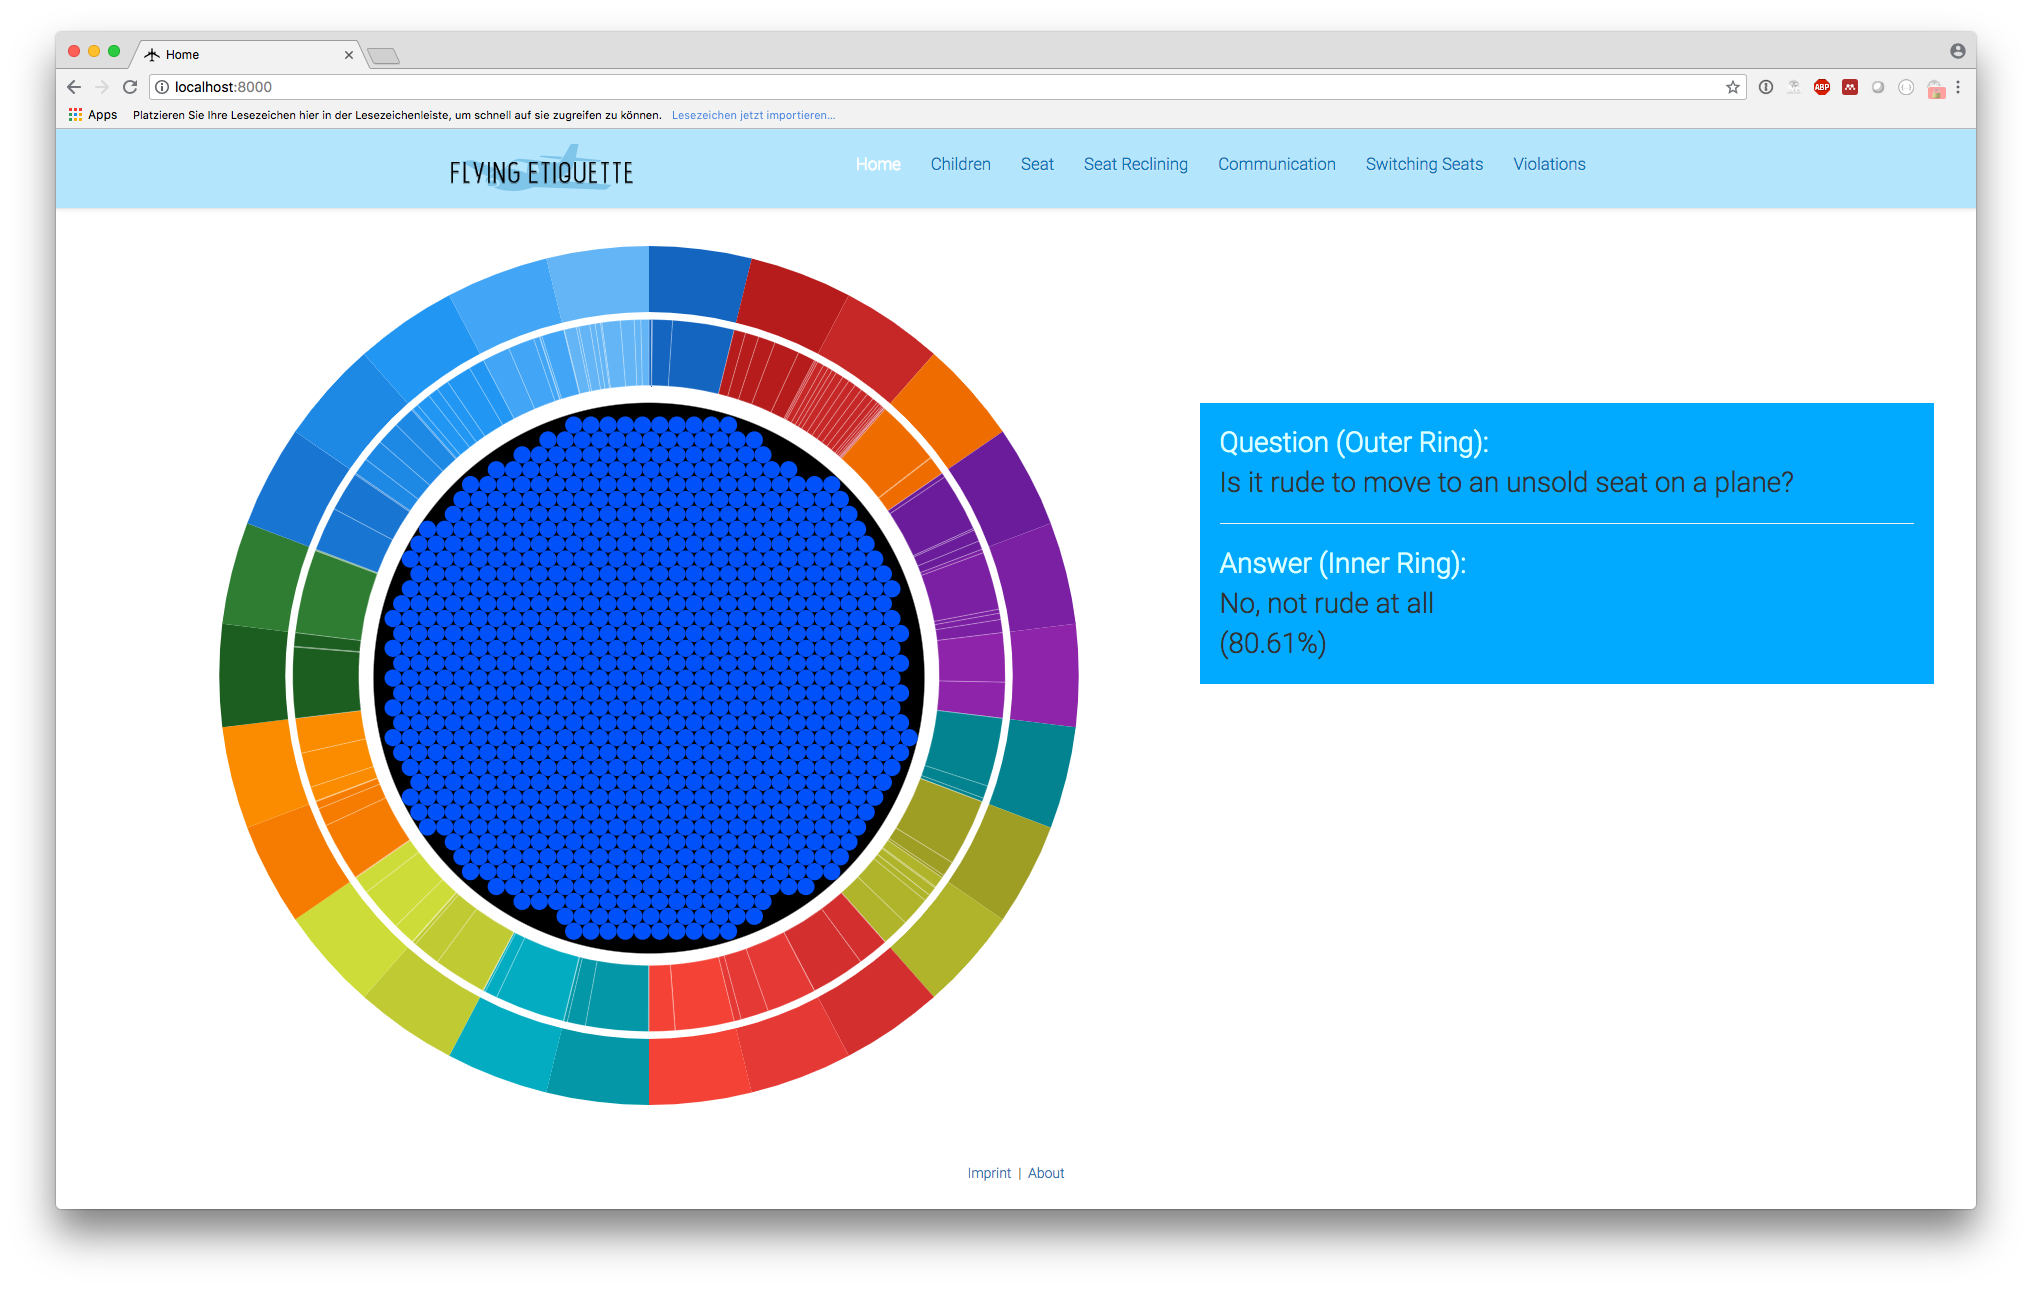
\includegraphics[scale=0.3]{assets/start_hover_rings.png}
\caption{Screenshot der Startseite \textit{Home} mit dem Hovern über Ringsegmenten des Startdiagramms}
\label{ScStartDiagramHover}
\end{figure}

\subsubsection{Antworten/Segmente des inneren Rings anklicken}
Der innere Ring stellt eine der wichtigsten Interaktionsmöglichkeiten für den Nutzer bereit. Dieser kann dort eine Antwort anklicken und bekommt alle Probanden, die durch die Kreise in der Mitte dargestellt werden, angezeigt, die in der Studie diese Antwort gegeben haben. Dabei ist es möglich gleich mehrere Segmente auszuwählen, woraufhin nur  Probanden/Kreise hervorgehoben werden, die alle diese Antworten in der Studie abgegeben haben. Somit kann ein Nutzer selbst untersuchen, welche Antwortkombinationen wie oft gegeben wurden und ob bestimmte Kombinationen überhaupt vorkommen. Alle vom Nutzer ausgewählten Segmente des inneren Rings werden dabei farblich von den restlichen Segmenten abgegrenzt, damit man immer weiß, welche Segmente man gerade ausgewählt hat. Ausgewählte Antworten kann man mit einem erneuten Klick darauf wieder abwählen. Ist keine Antwort ausgewählt oder falls kein Teilnehmer eine bestimmte Kombination aufweist, sind alle Kreise dunkelblau und somit inaktiv (Abbildung \ref{ScStartDiagramInnerRingClick}).
\begin{figure}
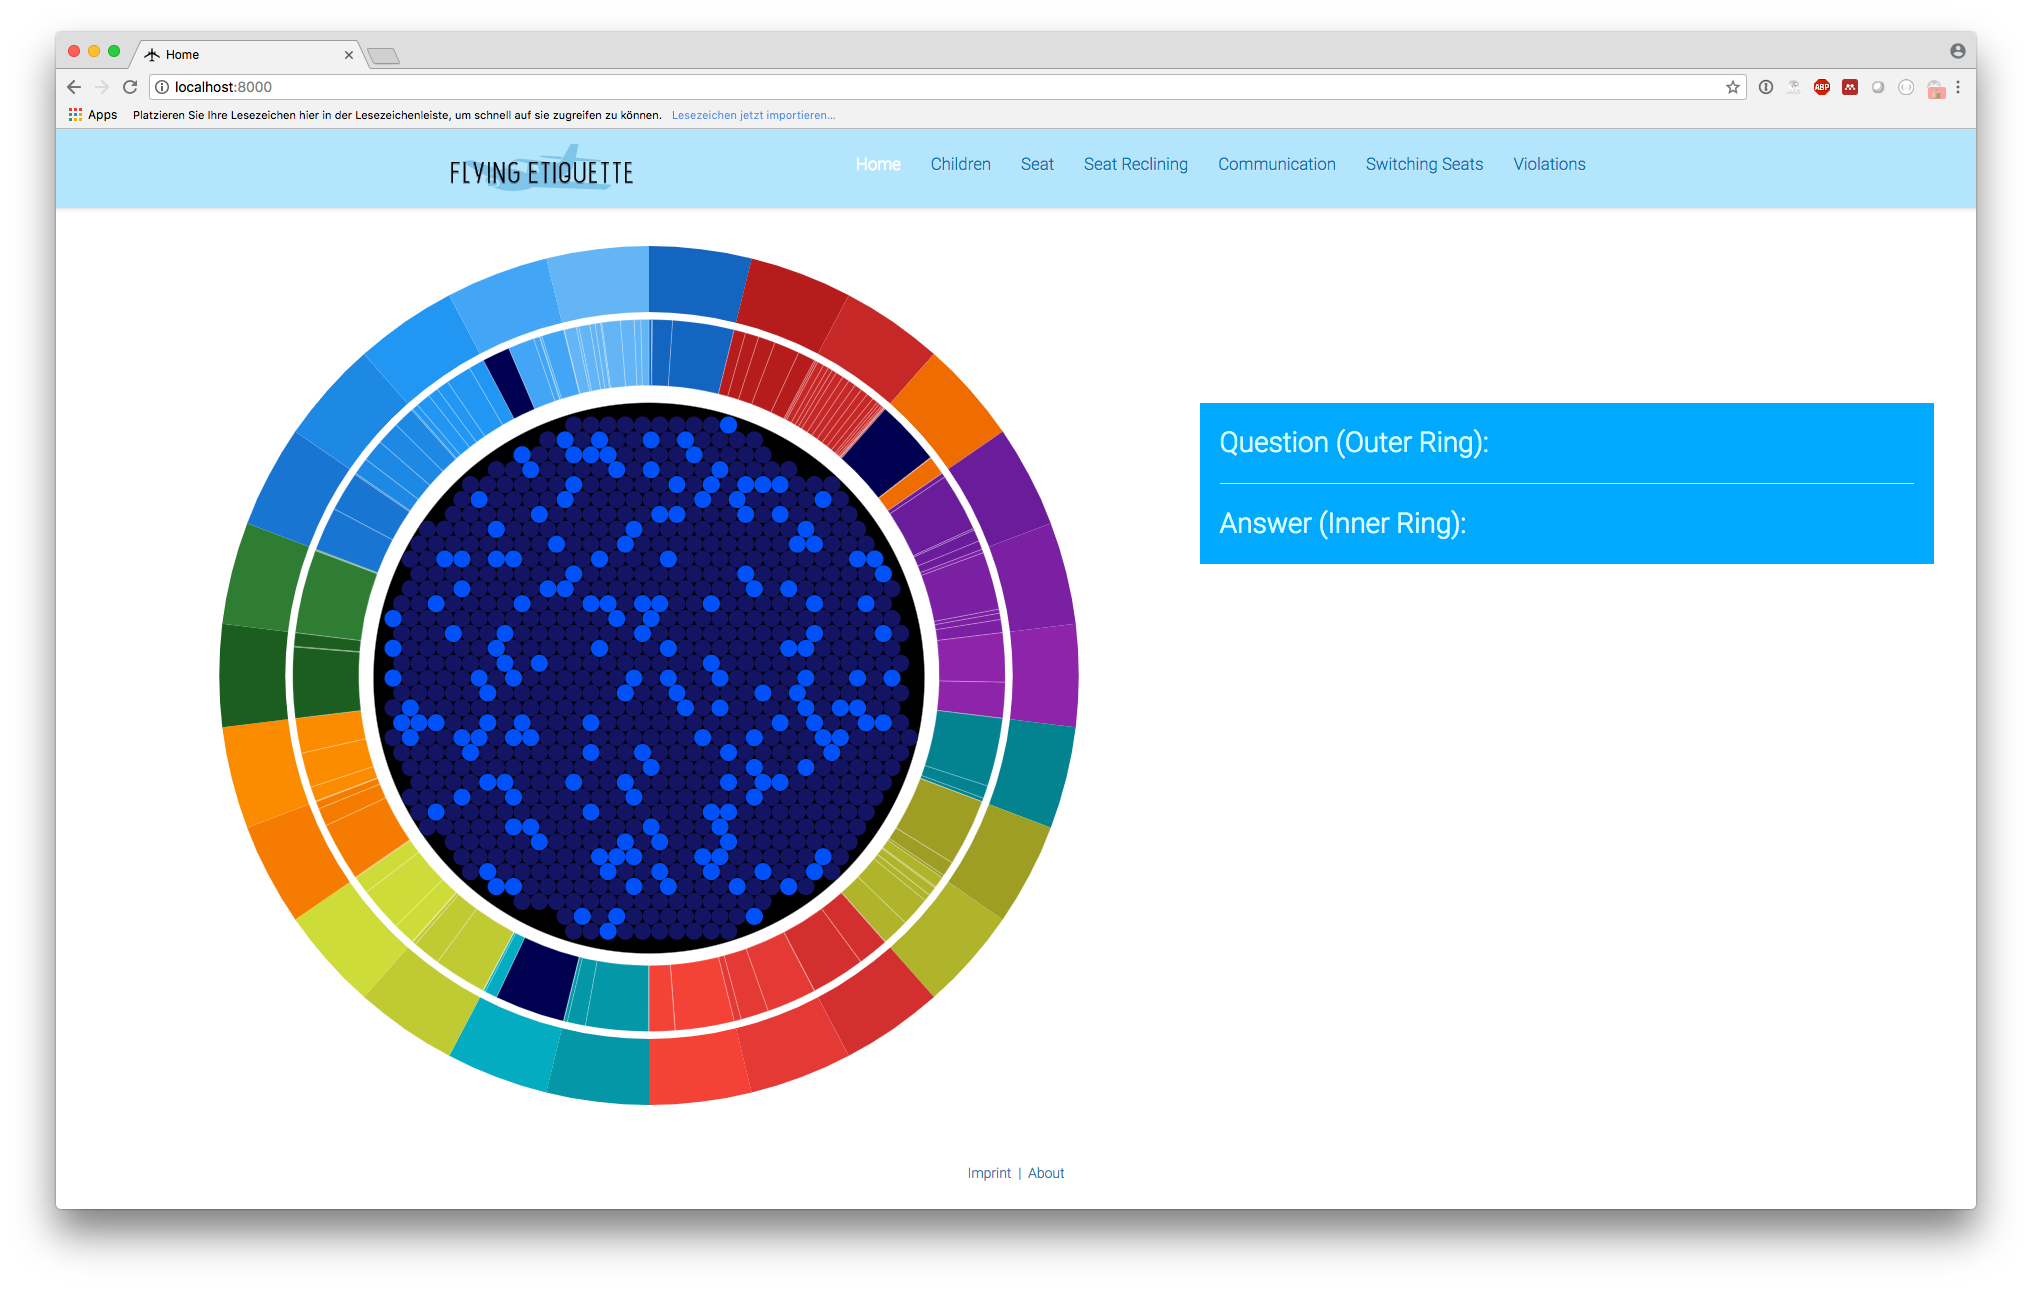
\includegraphics[scale=0.3]{assets/start_click_inner_ring_segments.png}
\caption{Screenshot der Startseite \textit{Home} mit dem Anklicken von mehreren Segmenten des Startdiagramms}
\label{ScStartDiagramInnerRingClick}
\end{figure}

\subsubsection{Zoom für inneren Ring}
Da einige der Antworten nur von wenigen Probanden gegeben wurden, erscheinen diese als sehr kleine Segmente des inneren Rings. Um diese besser sehen und für andere Interaktionsmöglichkeiten anklicken zu können, wurde ein Zoom eingebaut, mit dem man den inneren Ring mit Hilfe des Mausrads oder anderen entsprechenden Eingabemöglichkeiten vergrößern und wieder verkleinern kann. Der innere Ring kann dabei auch per Drag-and-Drop bewegt werden, falls der Zoom den restlichen Ring beim verkleinern verschiebt oder falls man andere Segmente bei der aktuellen Zoomgröße untersuchen will (Abbildung \ref{ScStartDiagramZoom}).
\begin{figure}
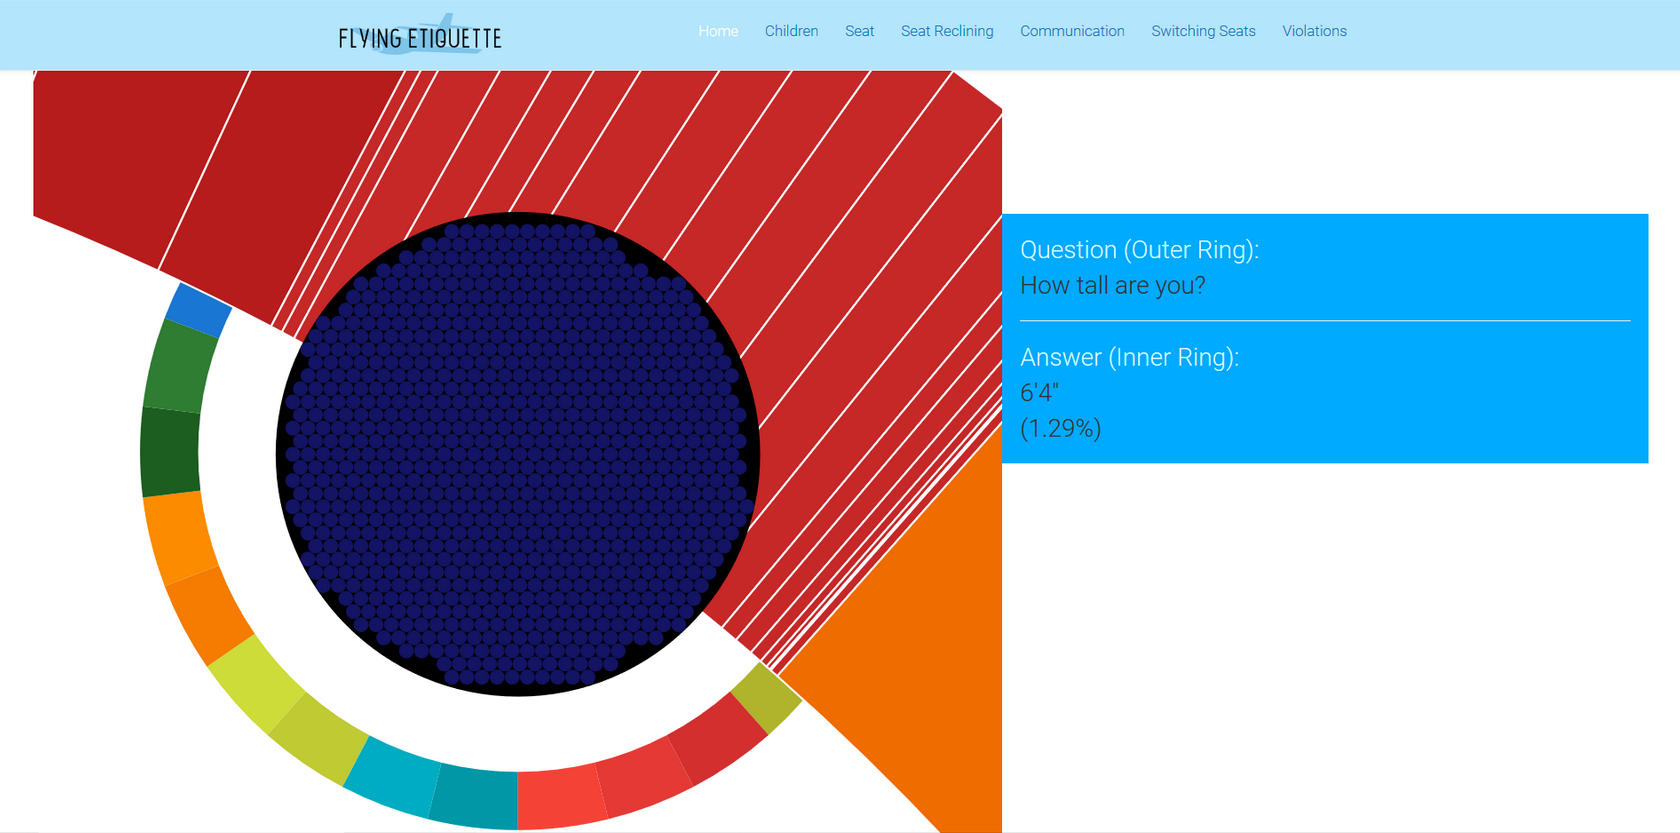
\includegraphics[scale=0.3]{assets/start_inner_ring_zoom.png}
\caption{Screenshot der Startseite \textit{Home} mit dem Zoom vom inneren Ring des Startdiagramms}
\label{ScStartDiagramZoom}
\end{figure}

\subsubsection{Probanden-Kreise anklicken}
Die Probanden-Kreise ermöglichen es für jeden Probanden dessen Antworten anzeigen zu lassen, indem der Nutzer auf einen der Kreise klickt. Daraufhin werden alle Segmente des inneren Rings, die den Antworten entsprechen, die der Nutzer angeklickt hat, farblich markiert. Somit ist es möglich, durch das Hovern über die markierte Segmente zu erfahren, welche Antworten dieser Proband gegeben hat. Die farbliche Darstellung vermeidet eine zu große Informationsflut an textueller Information, da einige der Fragen und Antworten sehr lang sind. Der aktuell ausgewählte Proband/Kreis wird in diesem Fall farblich hellblau hervorgehoben, während alle anderen Kreise inaktiv und somit dunkelblau werden (Abbildung \ref{ScStartDiagramDotClick}).
\begin{figure}
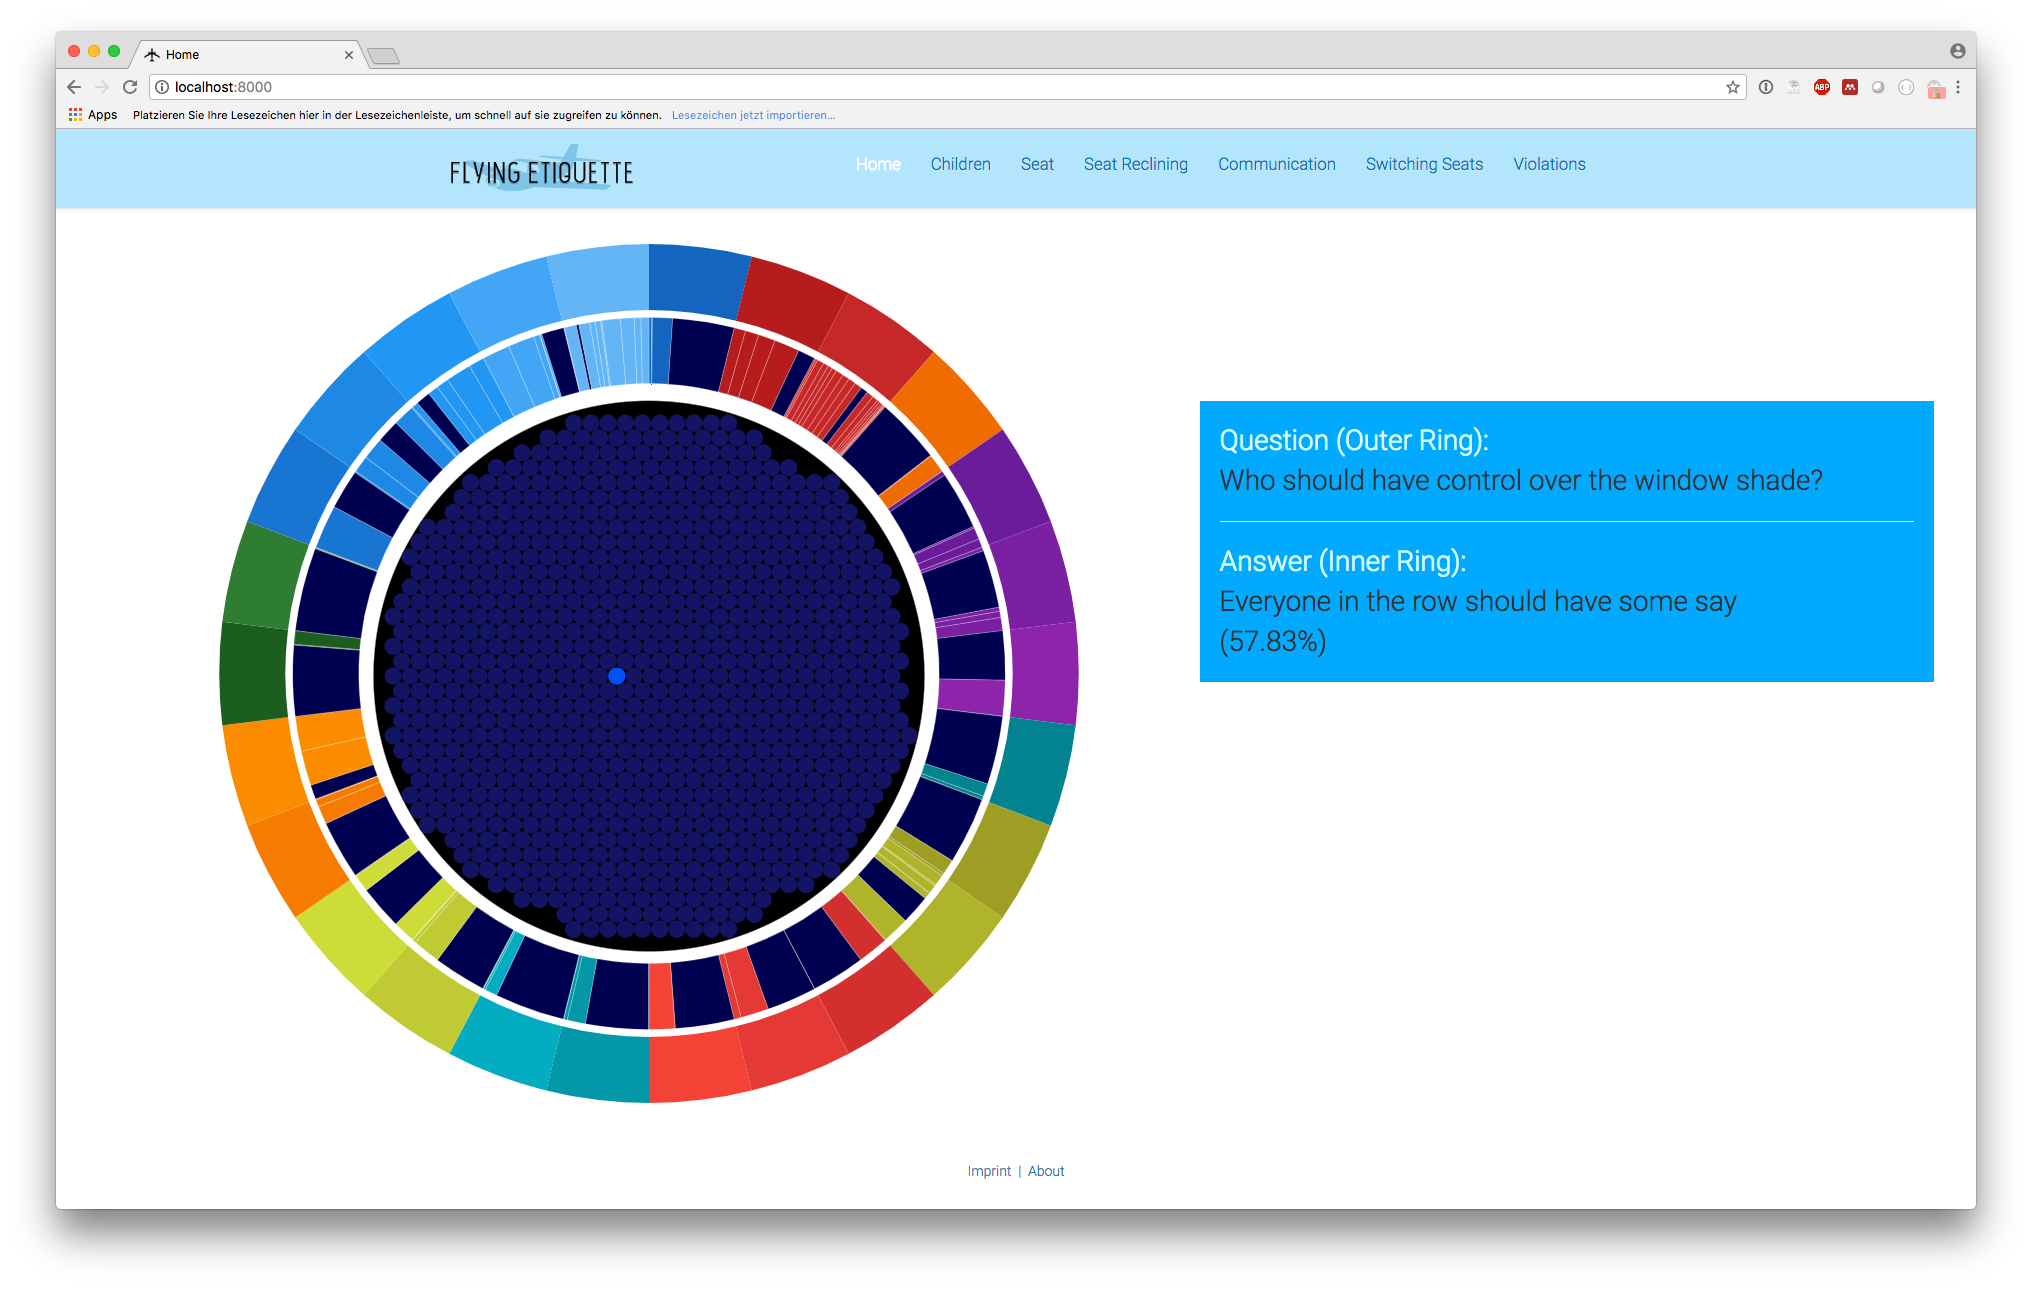
\includegraphics[scale=0.3]{assets/start_click_participant_dot.png}
\caption{Screenshot der Startseite \textit{Home} mit dem Anklicken eines Probanden-Kreises}
\label{ScStartDiagramDotClick}
\end{figure}

\section{Bubblediagramme}
Nachdem das Startdiagramm einen Überblick über die Daten geben sollte, geben die Bubblediagramme die Möglichkeit die in \ref{Datensatz} beschriebenen Kategorien genauer und interaktiv zu erforschen.
Die Wahl fiel auf Bubblediagramme, da der Nutzer hier auf einen Blick die Verhältnisse der gegebenen Antworten sehen kann. Die Größe der Bubbles spiegelt dabei immer die Anzahl der gegeben Antwort wider. Über den Bubbles befinden sich alle möglichen Antworten. Diese sind durch Linien mit der zugehörigen Bubble verbunden. Wenn der Nutzer über die Bubbles hovert, erscheint auf diesen die Anzahl der gegebenen Antworten und die Anzahl aller Antworten. So steht dem Nutzer neben der visuellen Größe der Bubbles, noch ein Zahlenwert zur Verfügung. 

Für jede Kategorie gibt es eine eigene Unterseite. Auf diesen befinden sich jeweils zwei bis drei Bubblediagramme, welche die Fragen der Kategorien repräsentieren. Jede Bubble steht für eine Antwort, die auf die jeweilige Frage geben werden konnte (Abbildung \ref{ScSwitchingSeats}). 
Die Grundfarbe eines Bubblediagramms ist dabei immer die Farbe, in welcher der Kreisabschnitt derselben Frage im Startdiagramm eingefärbt ist.
\begin{figure}
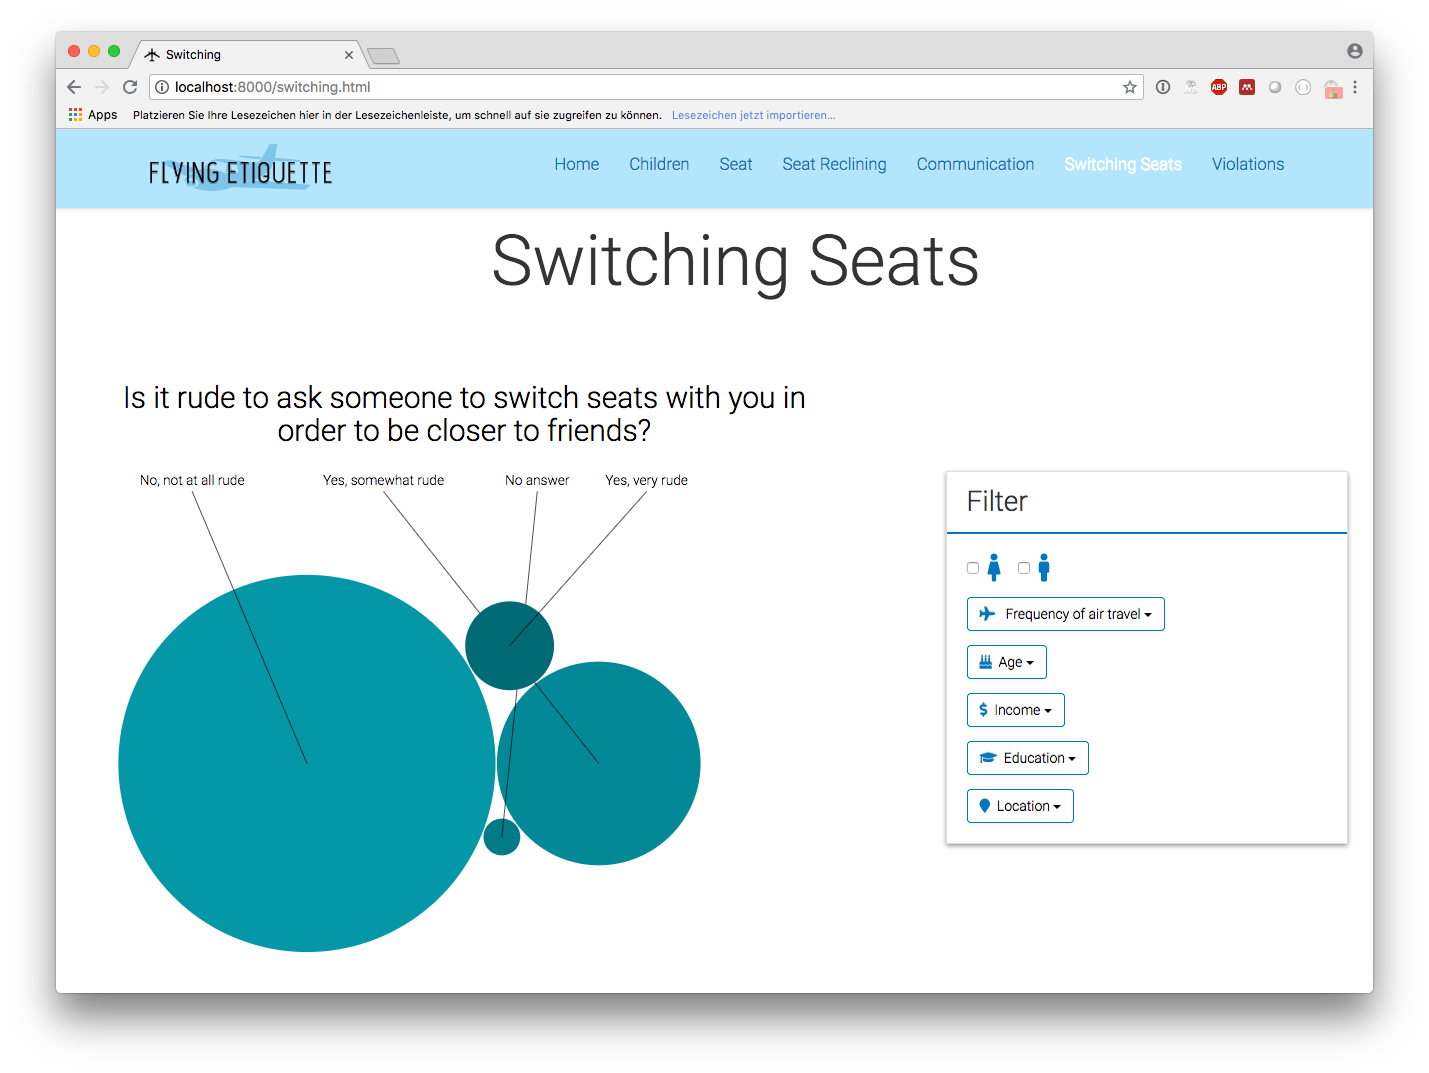
\includegraphics[scale=0.5]{assets/filter_standard.png}
\caption{Screenshot der Unterseite \textit{Switching Seats} mit Standard-Filtern}
\label{ScSwitchingSeats}
\end{figure}

\subsection{Filter}
Die Bubblediagramme können mit Hilfe von Filtern explorativ erforscht werden. Diese befinden sich jeweils rechts der Diagramme. Die Filter sind durch Icons und im Falle der Dropdown-Filter, durch einen kurzen Text gekennzeichnet. Die Wahl fiel auf Icons, da der Nutzer so sofort die Funktionalität des Filters erfassen kann. Ist das Icon aber trotzdem nicht eindeutig genug, kann der Nutzer zusätzlich über die Filter hovern und erhält dann eine genauere Erklärung, für was der jeweilige Filter steht. 

Werden die Filter gesetzt, passt sich die Größe der Bubbles an die Anzahl der gegebenen Antworten an. Das heißt die Bubbles sind anteilig immer so groß, wie die Anzahl der gegebenen Antworten. Das stellt sicher, dass der Nutzer auf einen Blick die Verhältnisse wahrnehmen kann (Abbildung \ref{ScSwitchingSeatsActive}).  
\begin{figure}
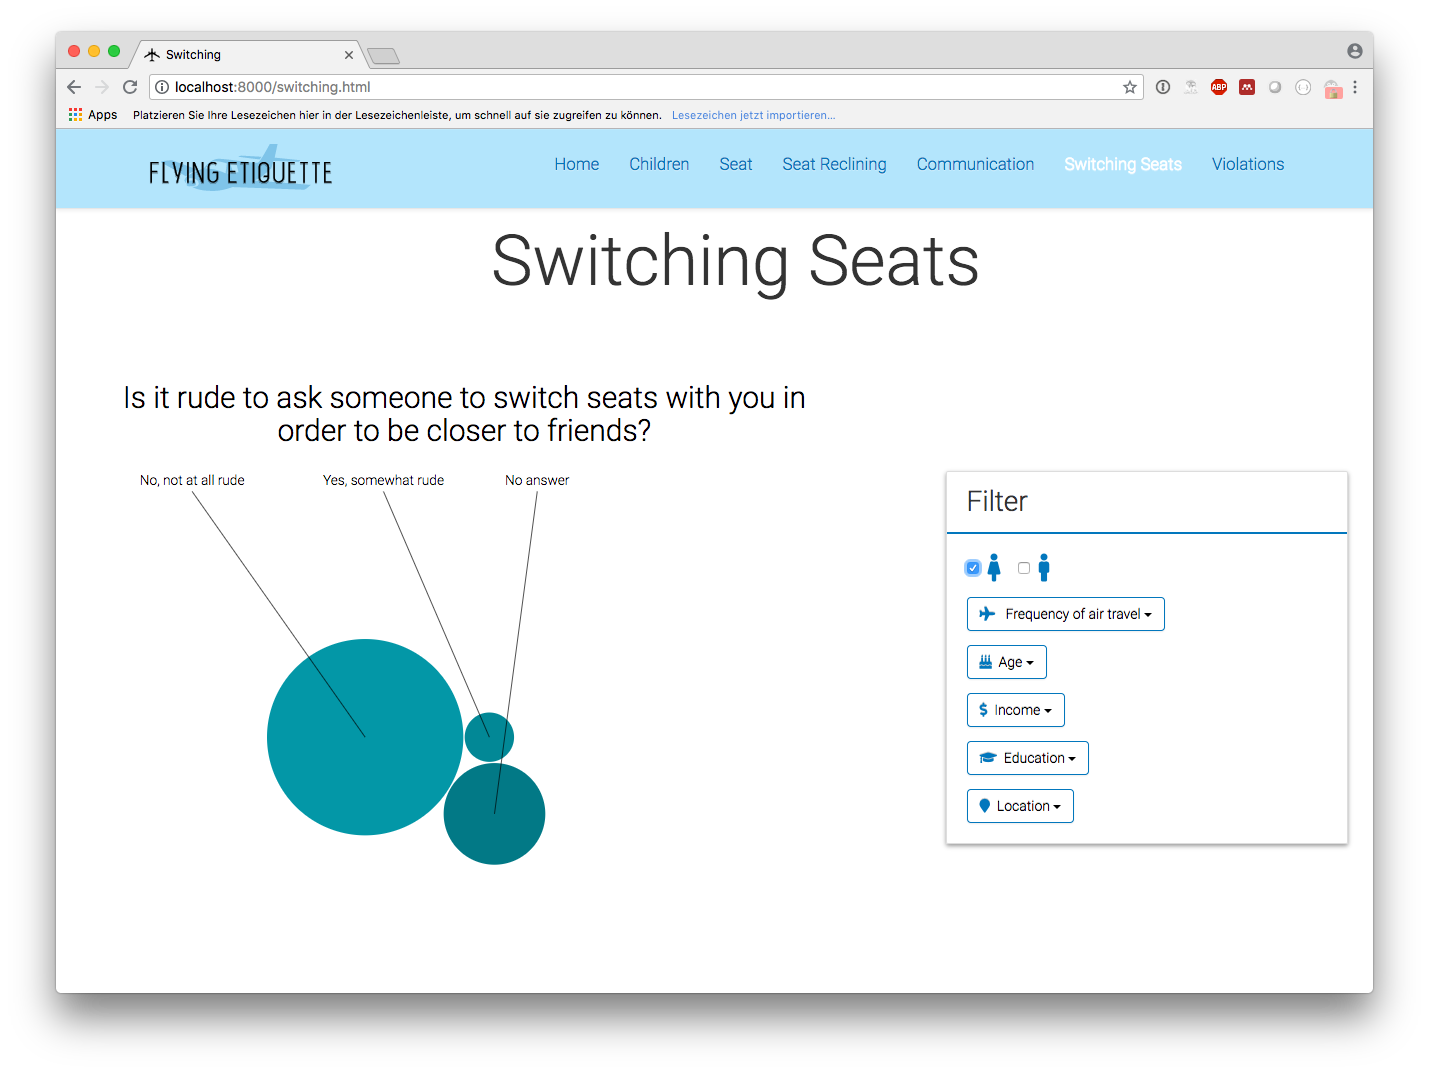
\includegraphics[scale=0.5]{assets/filter_standard_active.png}
\caption{Screenshot der Unterseite \textit{Switching Seats} mit aktiven Standard-Filtern}
\label{ScSwitchingSeatsActive}
\end{figure}
Es wird zwischen Standardfilter und speziellen Filtern, die nicht bei allen Diagrammen zur Verfügung stehen, unterschieden. Die Entscheidung spezielle Filter einzuführen fiel, da bestimmte Filter nur bei manchen Fragen Sinn machen. So macht es beispielsweise nur Sinn die Größe der befragten Person mit einzubeziehen, wenn absehbar ist, dass die Antwort auf eine Frage durch die Größe beeinflusst wird. Das ist beispielsweise bei der Frage der Fall, bei der erfasst wurde, wie unhöflich es ist, den Sitz im Flugzeug zurückzulehnen. Man kann davon ausgehen, dass es für größere Personen mit längeren Beinen wesentlich unangenehmer ist, wenn die Person vor ihr den Sitz zurücklehnt. Deshalb kann es bei dieser Frage sein, dass die Größe der befragten Person Einfluss auf die Antwort hat (Abbildung \ref{ScSeatRecliningActive}).
\begin{figure}
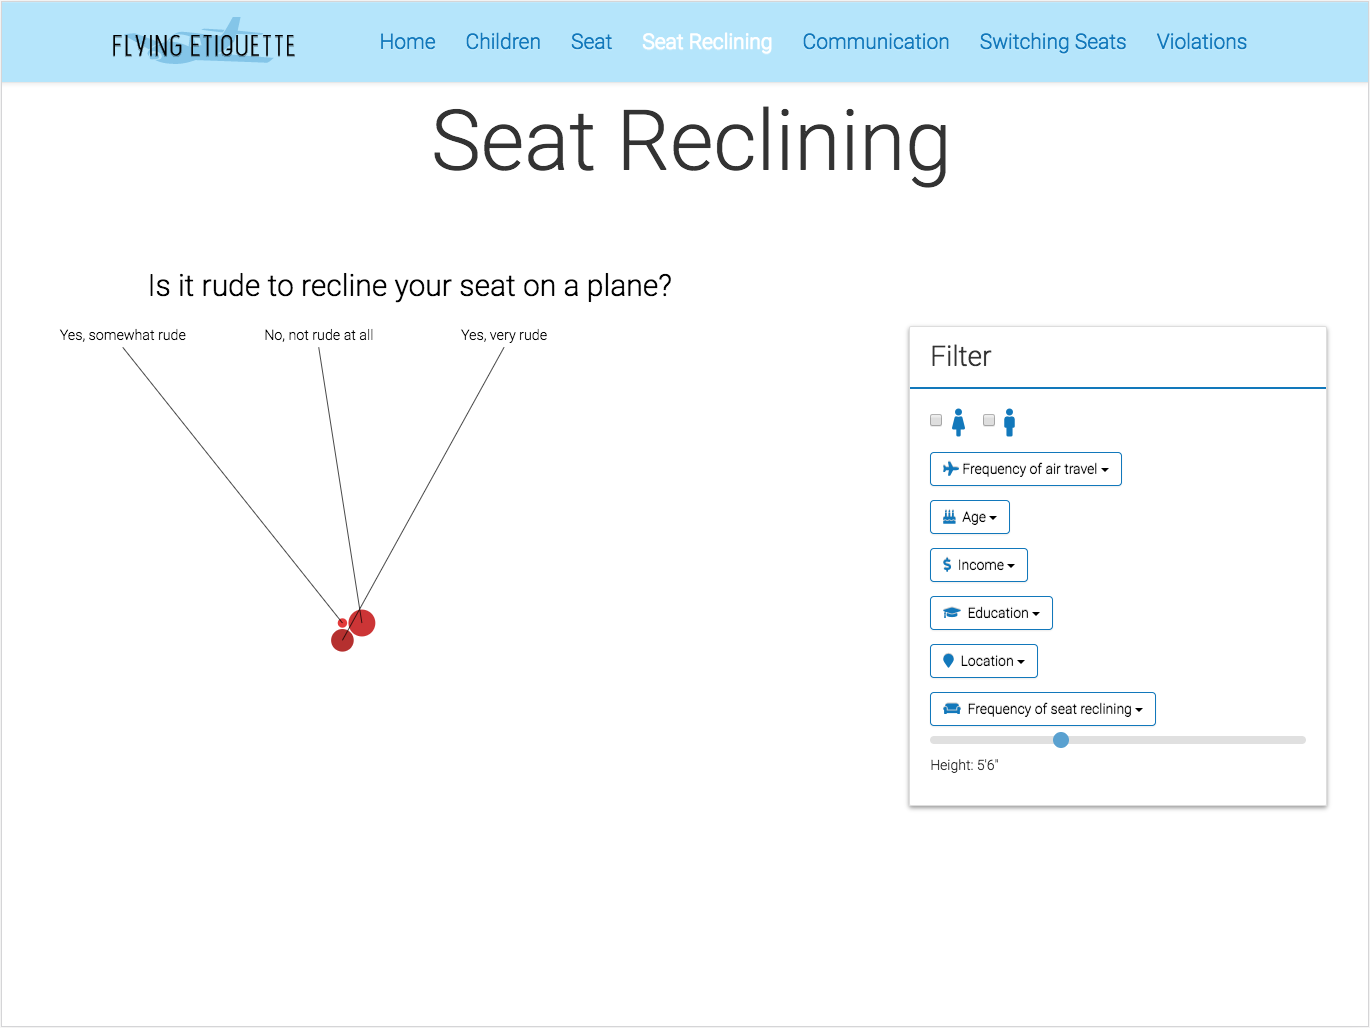
\includegraphics[scale=0.5]{assets/filter_seat_active.png}
\caption{Screenshot der Unterseite \textit{Seat Reclining} mit aktivem Grö{\ss}en-Filter}
\label{ScSeatRecliningActive}
\end{figure}

Folgende Standardfilter stehen bei allen Diagrammen zur Verfügung:
\begin{itemize}
\item Gender-Filter: Mit dem Gender-Filter kann nach dem Geschlecht, also nach männlich oder weiblich gefiltert werden.
\item FrequencyOfAirTravel-Filter: Mit dem FrequencyOfAirTravel-Filter kann nach der Häufigkeit, mit der die Testpersonen fliegen gefiltert werden. Zur Auswahl stehen: 
	\begin{itemize}
	\item Once a year or less
	\item Once a month or less
	\item A few times per month
	\item A few times per week
	\item Every day
	\end{itemize}
\item Age-Filter: Mit dem Age-Filter kann nach dem Alter der Testpersonen gefiltert werden. Zu Auswahl stehen: 
	\begin{itemize}
	\item 18 - 29
	\item 30 - 44
	\item 45 - 60
	\item > 60
	\end{itemize}
\item Income-Filter: Mit dem Income-Filter kann nach dem Jahreseinkommen der Testpersonen gefiltert werden. Zur Auswahl stehen: 
	\begin{itemize}
	\item \$0 - \$24,999
	\item \$25,000 - \$49,999
	\item \$50,000 - \$99,999
	\item \$100,000 - \$149,999
	\item \$150000
	\end{itemize}
\item Education-Filter: Mit dem Education-Filter kann nach dem höchsten Bildungsabschluss der Testpersonen gefiltert werden: Zur Auswahl stehen:
	\begin{itemize}
	\item High school degree
	\item Some college or Associate degree
	\item Graduate degree
	\item Bachelor degree
	\end{itemize}
\item Location-Filter: Mit dem Location-Filter kann nach der Region der USA, aus der die Testpersonen kommen gefiltert werden. Zur Auswahl stehen:
	\begin{itemize}
	\item New England
	\item East North Central
	\item East South Central
	\item West North Central
	\item West South Central
	\item Middle Atlantic
	\item South Atlantic
	\item Mountain
	\item Pacific
	\end{itemize}
\end{itemize}

Zusätzlich zu den Standardfiltern stehen auf zwei Unterseiten Sonderfilter zur Verfügung. 

Auf der Unterseite \textit{Children} ein Child-Filter, mit dem danach gefiltert werden kann, ob die Testpersonen mindestens ein Kind unter 18 Jahren haben. 

Auf der Unterseite \textit{Seat Reclining} stehen folgende zwei Sonderfilter zur Verfügung: 
\begin{itemize}
\item FrequencyOfeatReclining-Filter: Mit dem FrequencyOfeatReclining-Filter kann nach der Häufigkeit mit der die Testpersonen ihren Sitz zurücklehnen gefiltert werden. Zur Auswahl stehen:
	\begin{itemize}
	\item Never
	\item Once in a while
	\item About half the time
	\item Usually
	\item Always
	\end{itemize}
\item Height-Filter: Mit dem Height-Filter kann nach der Größe der Testpersonen gefiltert werden. Dabei können auf einem Slider Größen vom 5 Fuß bis größer als 6 Fuß und 6 Zoll gesetzt werden.
\end{itemize} 

\section{Aufteilung}
Link zum Git-Hub Repository: \newline
\href{https://github.com/RiaRentnueg/IV_SoSe18_flying-etiquette}{https://github.com/RiaRentnueg/IV\_SoSe18\_flying-etiquette}
\linebreak \newline
Kevin Angermeyer (Verantwortlich für das komplette Startdiagramm):
\begin{itemize}
\item Startdiagramm-Konzept testen und umsetzen
\item Kompletter Code für StartDiagramManager, StartDiagramController und StartDiagramModel 
\item Kleinere Anpassungen an der css- sowie index-Datei
\item Visuelle Darstellung des Startdiagramms auf der Startseite
\end{itemize}

\end{document}
